\documentclass[twoside]{article}

%\usepackage{aistats2021}
% If your paper is accepted, change the options for the package
% aistats2021 as follows:
%
\usepackage[accepted]{aistats2021}
\usepackage{amsfonts}
\usepackage{graphicx}
\usepackage{multirow}
%
% This option will print headings for the title of your paper and
% headings for the authors names, plus a copyright note at the end of
% the first column of the first page.

% If you set papersize explicitly, activate the following three lines:
%\special{papersize = 8.5in, 11in}
%\setlength{\pdfpageheight}{11in}
%\setlength{\pdfpagewidth}{8.5in}

% If you use natbib package, activate the following three lines:
\usepackage{natbib}
%\renewcommand{\bibname}{References}
%\renewcommand{\bibsection}{\subsubsection*{\bibname}}

% If you use BibTeX in apalike style, activate the following line:
%\bibliographystyle{apalike}

\begin{document}

% If your paper is accepted and the title of your paper is very long,
% the style will print as headings an error message. Use the following
% command to supply a shorter title of your paper so that it can be
% used as headings.
%
%\runningtitle{I use this title instead because the last one was very long}

% If your paper is accepted and the number of authors is large, the
% style will print as headings an error message. Use the following
% command to supply a shorter version of the authors names so that
% they can be used as headings (for example, use only the surnames)
%
%\runningauthor{Surname 1, Surname 2, Surname 3, ...., Surname n}

\twocolumn[

\aistatstitle{TDHNN: Time-Dependent Hamiltonian Neural Networks }

\aistatsauthor{ Shaan A. Desai$^{1,2}$ \And David Sondak$^{2}$ \And  Marios Mathiakis$^{2}$ }

\aistatsaddress{ Machine Learning Research Group \\University of Oxford $^1$ \And Institute of Applied Computational Science \\ Harvard University $^2$ } ]


\bibliographystyle{abbrv}
\begin{abstract}

Deep networks embedded with physically-informed priors demonstrate  remarkable performance in accurately learning and predicting non-linear dynamical systems. In particular, energy-conserving networks designed to exploit the Hamiltonian formalism show strong and consistent performance in learning autonomous systems that depend implicitly on time. Here, we extend this work to include an explicit time-dependence that generalizes the learning to non-autonomous dynamical systems. We achieve this generalisation by embedding the port-Hamiltonian formalism into our neural network. We show that such a system can learn complex forced and damped dynamics, including the chaotic duffing equation, while maintaining strong performance in settings with no explicit time-dependence.

%Unlike vanilla Artificial Neural Networks, Neural Networks embedded with physically-informed priors achieve remarkable results in accurately learning and predicting non-linear dynamical systems.
% despite this success, their generalization is often limited by the available training data which in practice only consists of a few short-range trajectories. naturally we might ask how we can generalize to unseen timesteps better?
% Despite this success, their generalization performance is often limited to short-range trajectories that run for less than the final training time. The performance degradation is due to state and energy drift induced by errors accumulating over time and it poses a critical challenge to learning highly non-linear and chaotic long-range dynamics precisely when data for only a limited number of short-range trajectories are available. One proposed solution to this challenge has been to incorporate symplectic integrators that aim to preserve the symplectic flow. Here, we present an alternative, an L1 penalty of the Hamiltonian derivative with respect to time: $d\mathcal{H}(p,q,t)/dt$. The inclusion of this term, a straightforward addition to the network, enforces the Hamiltonian to remain constant in time for a given trajectory. We empirically illustrate the stabilising effect this penalty has on our network. In addition, we use it solve problems in non-linear dynamics such as heinon-heiles, 3-body problem and double pendulum.
\end{abstract}

\begin{figure*}[ht!]
\centering
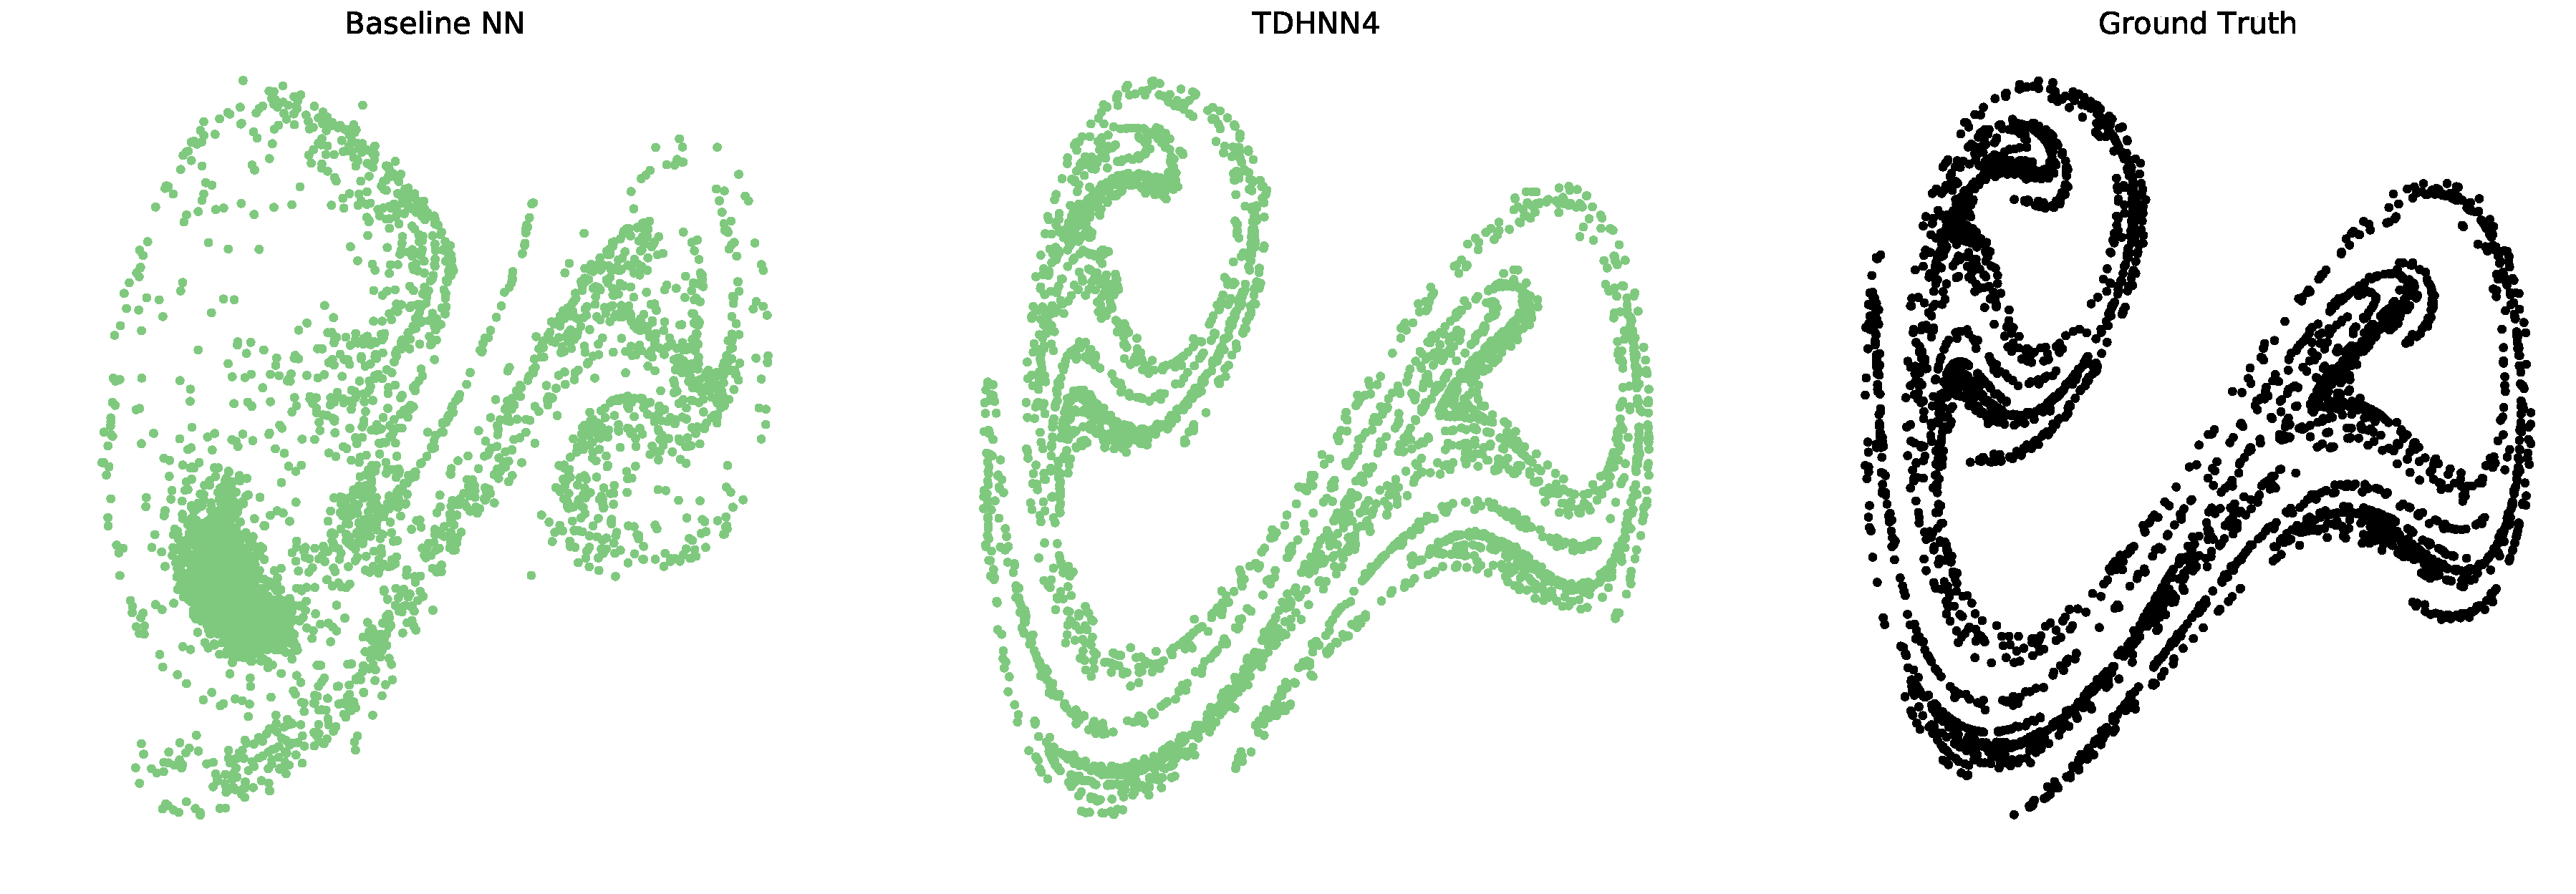
\includegraphics[width=0.9\textwidth]{figures/main_fig.pdf}
\caption{Poincar\'e Sections of a duffing oscillator in a chaotic regime. Both Baseline NN and TDHNN4 are trained for 20000 iterations with 2000 data points. TDHNN4 significantly outperforms Baseline NN at recovering the ground truth Poincar\'e section.}
\end{figure*}
\label{fig.chaos}
\section{Introduction}

Neural networks, as universal function approximators, have shown resounding success across a host of domains. However, their performance in learning physical systems has often been limited. New research aimed at \textit{scientific machine learning} - a branch that tackles scientific problems with domain-specific ML, is paving a way to address these challenges. It has been shown that prior theoretical information embedded in networks, such as Hamiltonian mechanics \cite{greydanus} demonstrate a significant performance uplift in learning. This excitement has spurred others to work with Lagrangians, ODEs and even graphs in order to tackle the learning of dynamical systems. Despite their widespread adoption, a major bottleneck of many of the existing methods is the lack of an explicit-time dependence as is evident across a host of forced dynamical systems. The most general form of Hamilton's equations, includes an explicit time dependence term. We show that the addition of this term, coupled with a few intuitive regularizations can induce networks to learn from both autonomous and non-autonomous settings. We extensively benchmark this addition across multiple datasets and consistently find the inclusion to be of benefit. Furthermore, we emphasise that the constraint is an easy plug-and-play addition to existing networks and illustrate how existing networks such as HNN, Symp ODEN and Hnets benefit from its inclusion. 

\begin{figure}[h!]
\centering
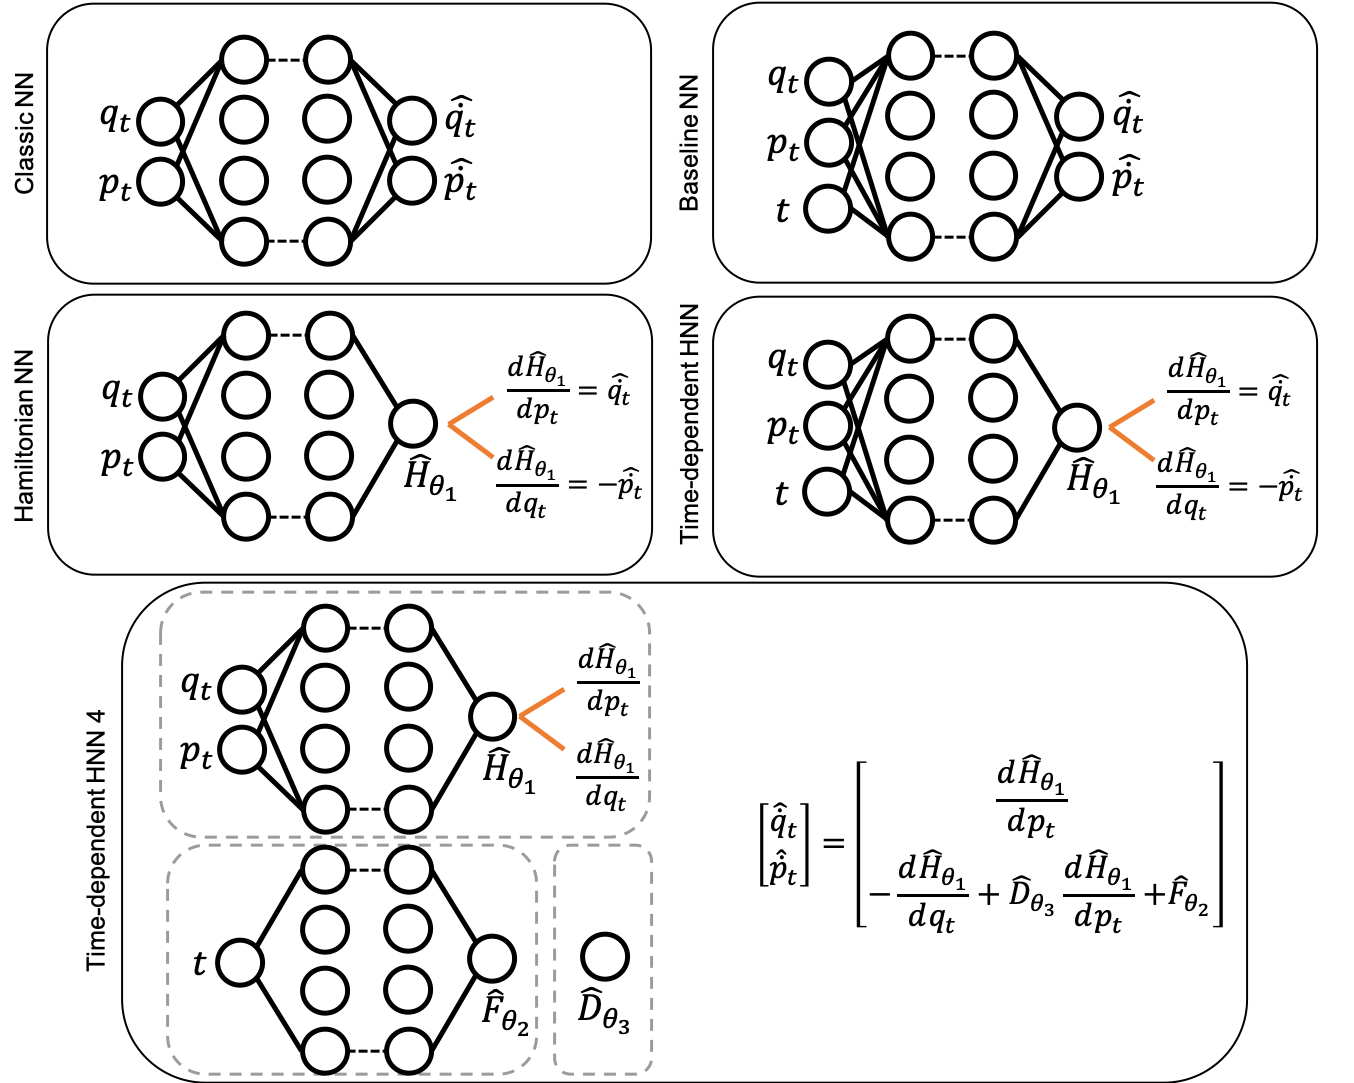
\includegraphics[width=0.4\textwidth]{figures/architect.png}
\caption{Architectures used to learn dynamics in this paper. The naive extension of classic NN and Hamiltonian NN (top left) is to incorporate time as an additional input variable (top right). Our innovation, which exploits Port-Hamiltonians, explicitly learns the force $F_{\theta_2}$ as well as the damping coefficient $D_{\theta_3}$.}
\label{fig.architecture}
\end{figure}

\section{Background}

\subsection{Hamiltonian Neural Networks}

Recently, \cite{greydanus_hamiltonian_2019} demonstrated that dynamic predictions through time can be improved using Hamiltonian Neural Networks (HNNs) which endow models with a Hamiltonian constraint. The Hamiltonian is an important representation of a dynamical system because it is one of two well-known approaches that generalizes classical mechanics. The Hamiltonian $\mathcal{H}$ is a scalar function of position $\mathbf{q} = (q_1,q_2,....,q_M)$ and momentum $\mathbf{p} = (p_1,p_2,....,p_M)$. It is a powerful representation because it allows us to obtain the time derivatives of the inputs $(\dot{q},\dot{p})$ by simply differentiating the Hamiltonian with respect to its inputs (see Eqn. \ref{eqn.hamiltonian}.)
\begin{equation}
\frac{\mathrm{d}\mathbf{q}}{\mathrm{d}t} = \frac{\partial \mathcal{H}}{\partial \mathbf{p}}, ~~~
\frac{\mathrm{d}\mathbf{p}}{\mathrm{d}t} = -\frac{\partial \mathcal{H}}{\partial \mathbf{q}}
\label{eqn.hamiltonian}
\end{equation}
As a consequence, it is noted in \cite{greydanus_hamiltonian_2019} that by parametrizing the Hamiltonian with a neural network e.g. $H_{\theta}(\mathbf{q},\mathbf{p})$ where $\theta$ represents a deep neural network, one can easily obtain the system's dynamics by differentiating (via autograd) the Hamiltonian with its inputs. This information allows us to build two 1st-order differential equations which can be used to update the state space, $(\mathbf{q},\mathbf{p})$. Equation \ref{eqn.action_int} shows this integral, in which we define the symplectic gradient $\mathbf{S}  = \left [ \frac{\partial \mathcal{H}}{\partial \mathbf{p}},-\frac{\partial \mathcal{H}}{\partial \mathbf{q}} \right ] $:
\begin{equation}
(\mathbf{q},\mathbf{p})_{t+1} = (\mathbf{q},\mathbf{p})_t + \int_t^{t+1} \mathbf{S}(\mathbf{q},\mathbf{p}) \mathrm{d}t
\label{eqn.action_int}
\end{equation}
However, this is not the only benefit in learning a Hamiltonian. Another key attribute of the Hamiltonian is that the vector field $\mathbf{S}$ is a symplectic gradient meaning $\mathcal{H}$ remains constant as long as state vectors are integrated along $\mathbf{S}$. This result links the Hamiltonian with the total energy of the system such that $\mathcal{H}(\mathbf{q},\mathbf{p}) = E_{tot}$ for many physical systems. Therefore, the Hamiltonian is a powerful inductive bias that can be utilised to evolve a physical state while maintaining energy conservation. 

Although this formalism is compact and powerful, it does not readily generalize to damped or forced system. As such, we refer to port-Hamiltonian systems.

\subsection{Port-Hamiltonians}

Port-Hamiltonians are a formalism that allow us to incorporate damping and forcing terms. One formalism outlined in \cite{dissipative sympoden} shows how to represent a general form for such a system. We extend that work to include time-dependent forcing and eliminate the need for an explicit control input $u$. This results in the following equation:
\begin{equation}
\resizebox{0.9\linewidth}{!}{$%
\begin{bmatrix}
\dot{\mathbf{q}} \\
\dot{\mathbf{p}}
\end{bmatrix}
=
\Bigg(\begin{bmatrix}
0 & \mathbf{I} \\
-\mathbf{I} & 0
\end{bmatrix} +
\begin{bmatrix}
0 & 0 \\
0 & \mathbf{D}_{\theta_2}(\mathbf{q})
\end{bmatrix}
 \Bigg)
 \begin{bmatrix}
\frac{\partial \mathcal{H}_{\theta_1}}{\partial \mathbf{q}} \\
\frac{\partial \mathcal{H}_{\theta_1}}{\partial \mathbf{p}}
\end{bmatrix}
+
\begin{bmatrix}
0 \\
\mathbf{g}(\mathbf{q})
\end{bmatrix}
F_{\theta_3}(t)
$%
}%
\end{equation}
where $\mathbf{D}_{\theta_2}(q)$ is the damping term and $g(q)F_{\theta_3}(t)$ is the forcing term. 

Given this general formalism, we make some simplifications. Here, instead of using a generalized semi-positive definite damping matrix, we simply aim at learning the lower right term which is most often independent of $\mathbf{q}$. As such, we parametrize $\mathbf{D}$ with a single, scalar learnable parameter. Secondly, for many physical systems, $g(q)$ is also a scalar quantity, so we abstract this scalar learning into $F(t)$ by setting $g(q) = 1$.

\section{Related Work}

Numerous recent methods show how to learn dynamics via physically informed priors:

Functional Form priors:
PINNs and Hamiltonian Nets (Marios) look at directly embedding the equations into the loss function. PINNs furthermore exploit autograd to compute partial-derivatives. 

Integrator focused:
NeuralODE - focuses on backprop through an embedded integrator
Symplectic networks


Graph based methods:
Battaglia et al emphasise relational inductive biases. Can show an ability to learn complex physics.

Lagrangian/Hamiltonian approaches:
DeLAN looks at embedding Lagrangians to learn robotic control

Recent advances:
CHNN, one of the most recent advances, looks at enforcing cartesian coordinate learning by adding holonomic constraints via lagrange multipliers instead of learning a fully implicit constraint in complex coordinate spaces


Combining inductive biases such as NeuralODE, graphs and Hamiltonians is presented in Hamiltonian Graph Networks and Variational Integrator Graph Networks.


\section{Method}

\begin{equation}
\resizebox{0.9\linewidth}{!}{$%
\mathcal{L} =\left\| \frac{\partial \mathcal{H}_{\theta_1}}{\partial \mathbf{q}} +  \frac{\partial \mathbf{p}}{\partial t} \right\| +\left\| \frac{\partial \mathcal{H}_{\theta_1}}{\partial \mathbf{p}} -  \frac{\partial \mathbf{q}}{\partial t} \right\|+ \alpha_{reg}| F_{\theta_3} (t)| + \beta_{reg}|D_{\theta_2}| 
$%
}
\end{equation}

To learn the dynamics, we feed in a state-vector $\mathbf{S}_t = [\mathbf{q},\mathbf{p},\mathbf{t}]$ to our model. The first neural-network consists of 3 hidden layers designed to predict $\mathcal{H}$ from $[\mathbf{q},\mathbf{p}]$ data. The second neural-network consists of a single weight parameter designed to learn the damping coefficient $\mathbf{D}$ and the third neural-network consists of 2 hidden layers designed to predict $\mathbf{F(t)}$ from t. We use an L2-norm penalty for the predicted state-vectors and an L1-norm for force and damping to encourage sparsity. We do this because we would like our networks to identify classical autonomous systems (which may not have force or time) as well as non-autonomous systems. For our experiments we use 200 hidden layers and find that most activations such as tanh, sin and cos yield comparable results. To benchmark our method, as \cite{greydanus} do, we use a baseline NN that takes in $S_t$ and predicts $[\dot{q},\dot{p}]$. We also take the straightforward extension of HNN to include time as a variable input. At inference, we use an Runge-Kutta 4th order integrator to rollout the initial conditions. 

\section{Results}

We benchmark the performance of our models on numerous datasets that canvas time-independent systems to complex chaotic forced systems.

\subsection{Simple Mass Spring}

The simple mass spring system is a well known system from classical physics that obeys Hooke's Law. The Hamiltonian for a simple mass spring system is written as:

\begin{equation}
\mathcal{H} = \frac{1}{2}kq^2 + \frac{1}{2m}p^2 
\end{equation}

For simplicity, we set $k$ and $m$ to 1 for our experiments. We sample 25 initial training conditions such that r in $q^2+p^2 = r^2$ is between 0.5 and 1.5.  The test error in fig.x is measured as a Mean squared error for 50 trajectories. The main motivation in learning this system is to show that learning a separate forcing term results in much better state and energy rollout in comparison to TDHNN and baseline NN. The main reason for this is that while TDHNN and baseline NN will learn dynamics with time-steps within the training regime, they typically cannot generalize to unseen timesteps. Learning a separate forcing term and regularizing keeps the time component independent of the Hamiltonian and therefore allows us to nearly match the performance of HNN.

\begin{figure}[h!]
\centering
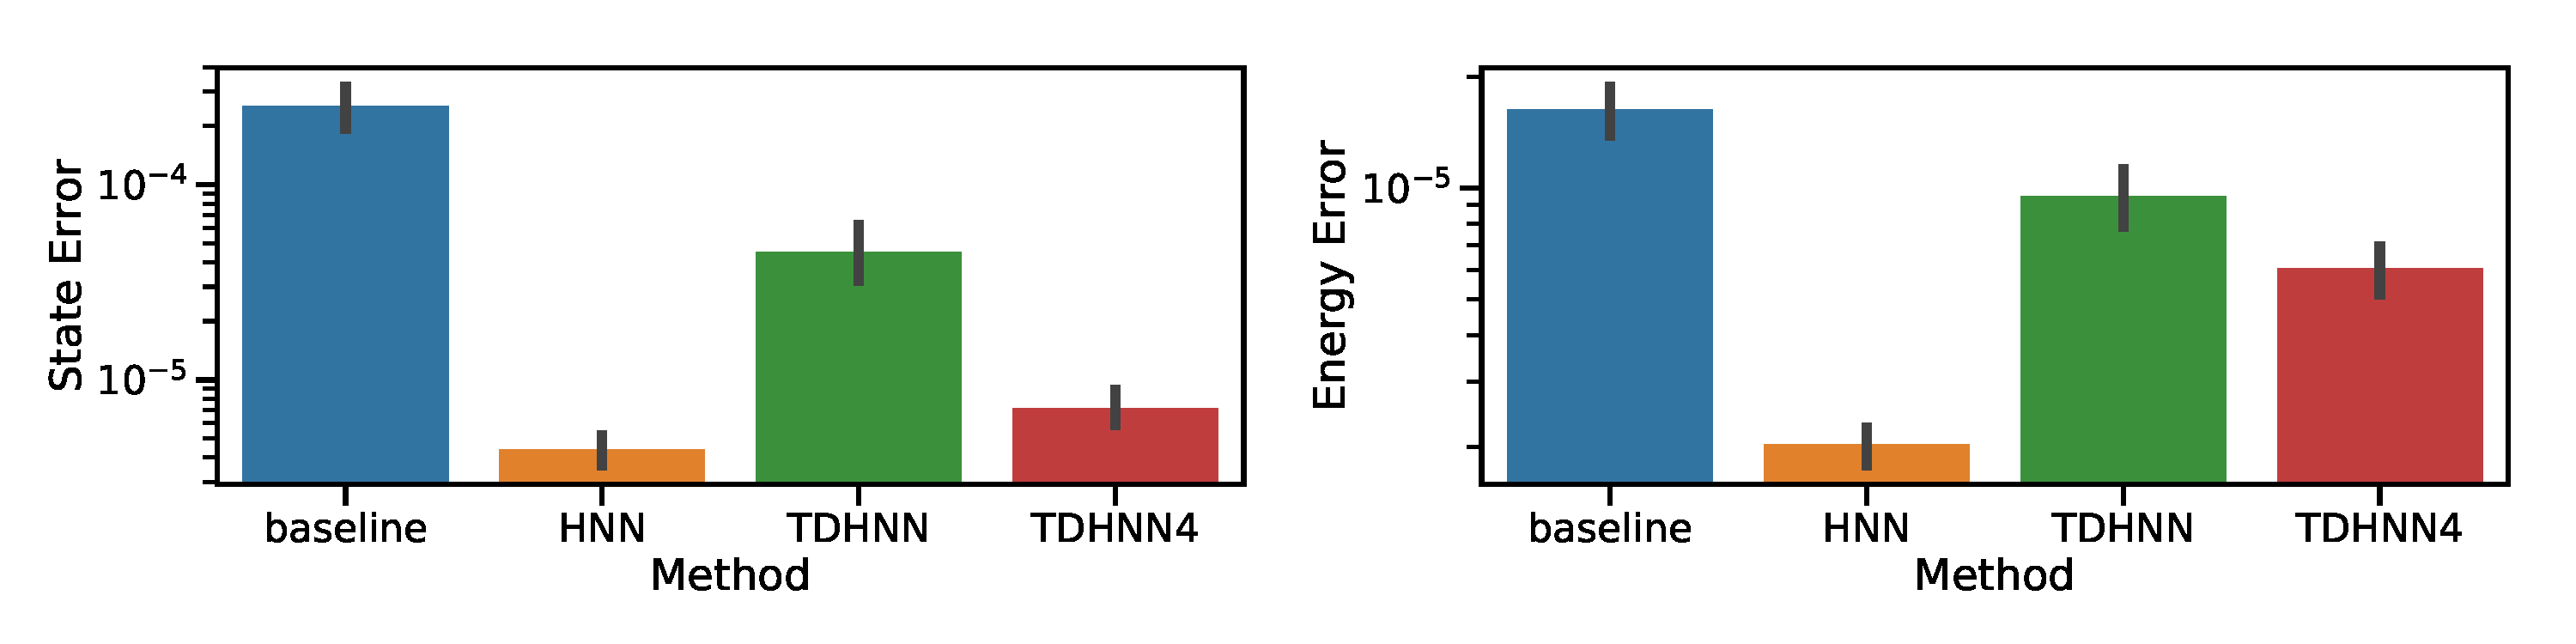
\includegraphics[width=0.5\textwidth]{figures/mass_spring_errors.pdf}
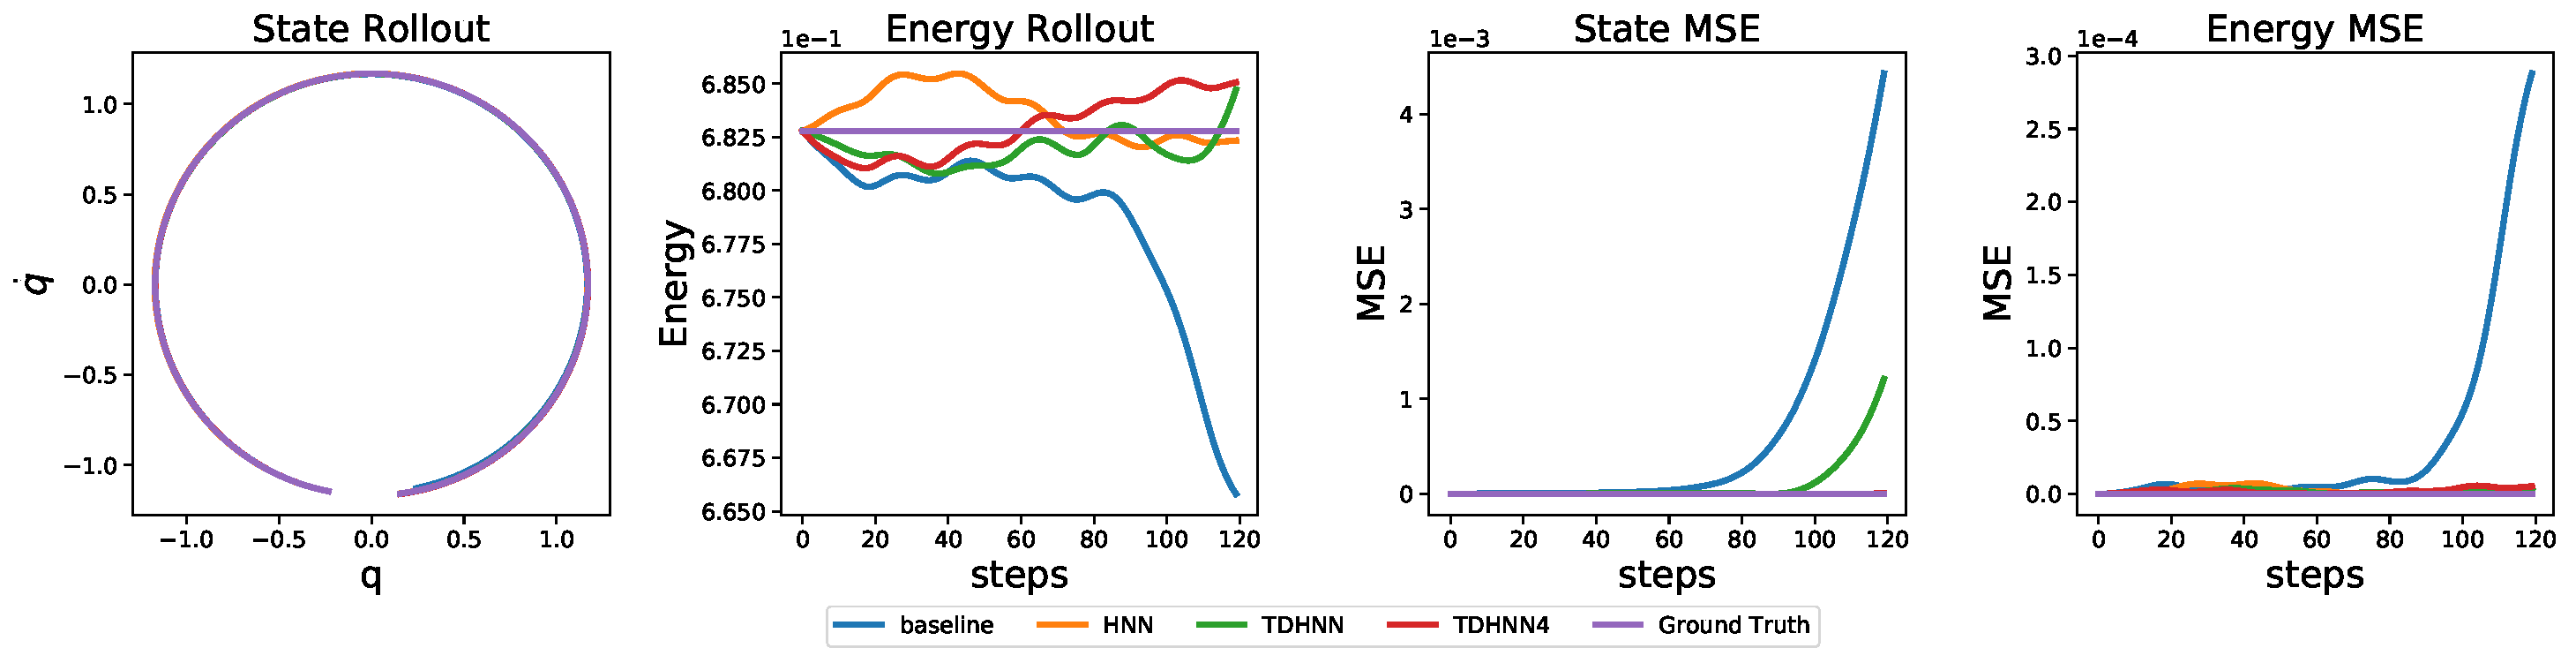
\includegraphics[width=0.5\textwidth]{figures/mass_spring_long.pdf}
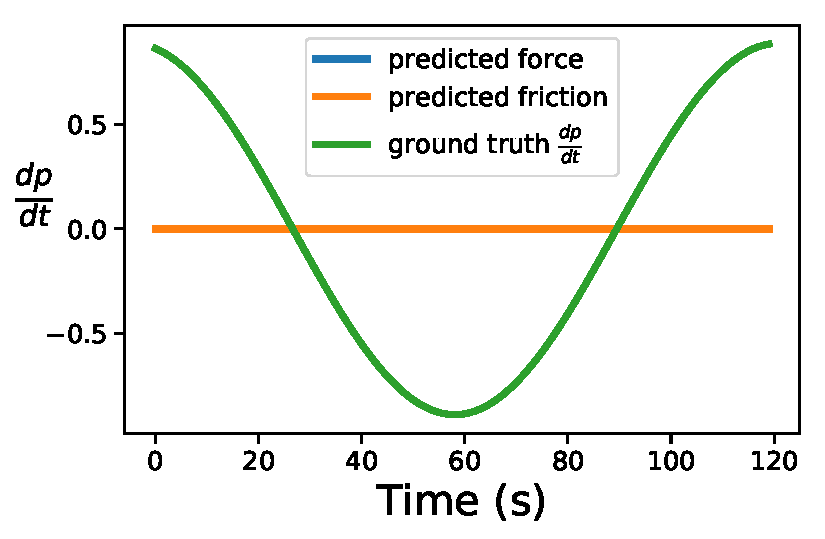
\includegraphics[width=0.4\textwidth]{figures/mass_spring_pred_force.pdf}
\caption{Simple Mass Spring system has no explicit time dependence. We see that TDHNN4 can almost recover the dynamics of HNN which doesn't depend on time. The result is achieved by regularising the force and friction terms as can be seen in the bottom figure. Baseline and TDHNN are unable to achieve the same state-error as their time-dependence }
\end{figure}


\subsection{Damped Mass Spring}

Damping/friction is generally not considered part of Hamiltonian systems. However, as we saw with Port-Hamiltonians, there is a straightforward way to account for the damping term. The time derivative of $\mathbf{S}_t$ is obtained by adding a damping coefficient to $\dot{\mathbf{p}}$. 

\begin{figure}[h!]
\centering
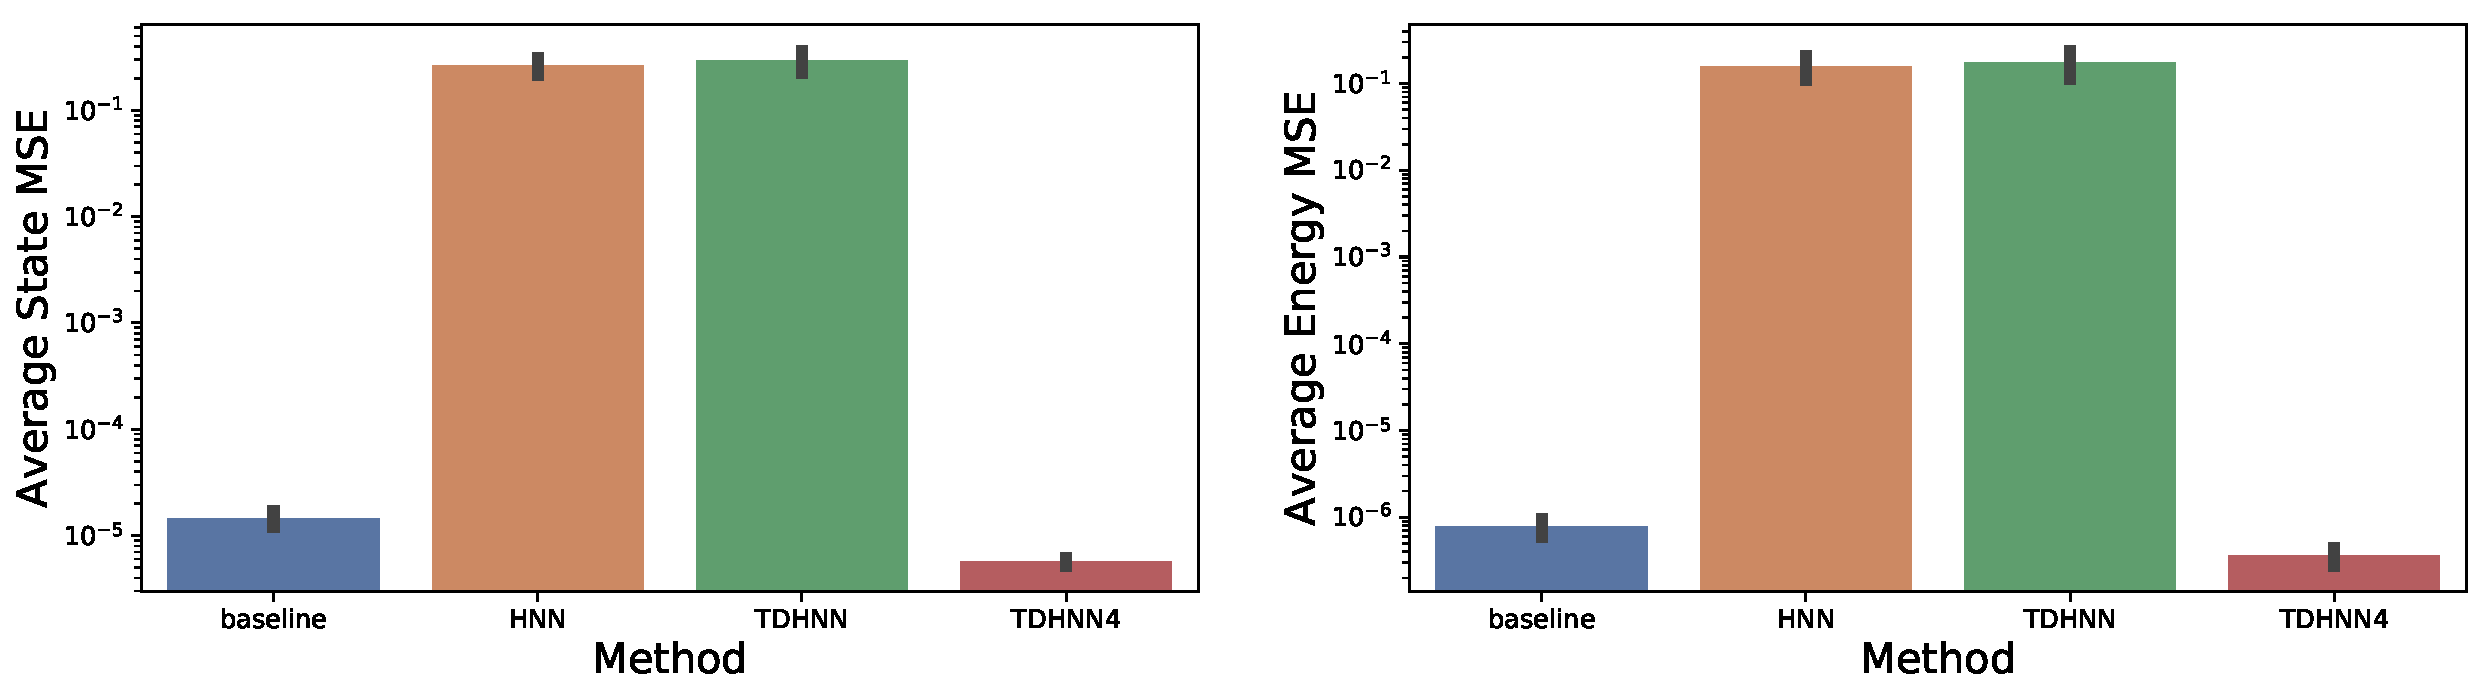
\includegraphics[width=0.5\textwidth]{figures/damped_1_errors.pdf}
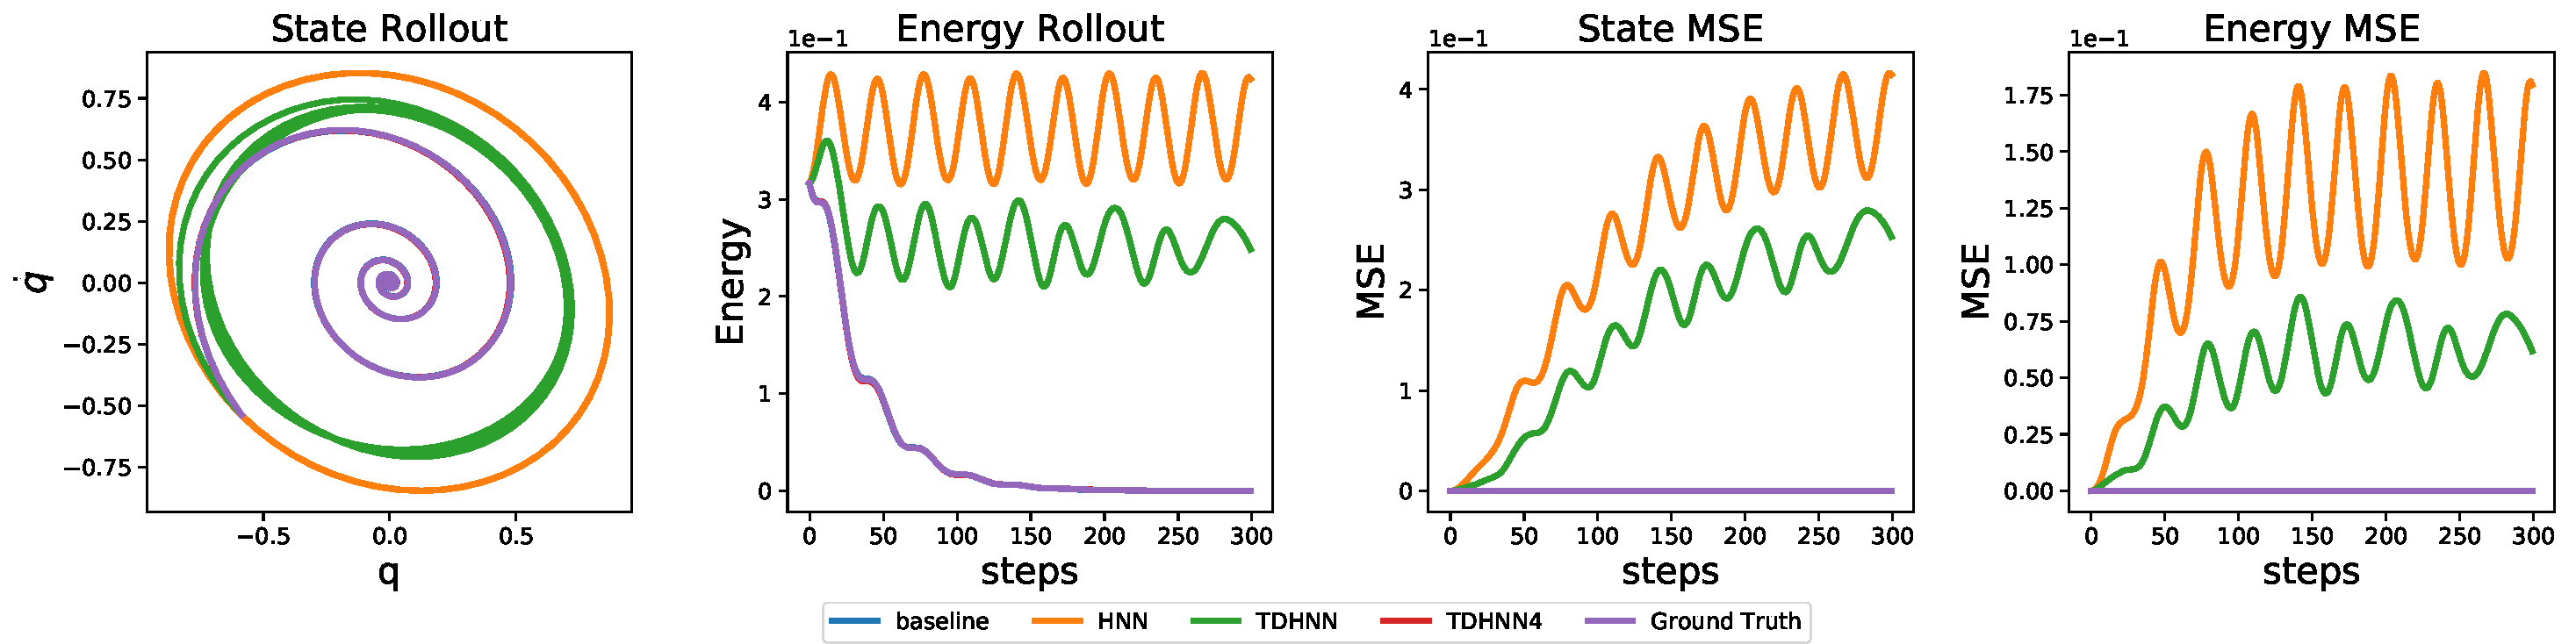
\includegraphics[width=0.4\textwidth]{figures/damped_1_pred.pdf}
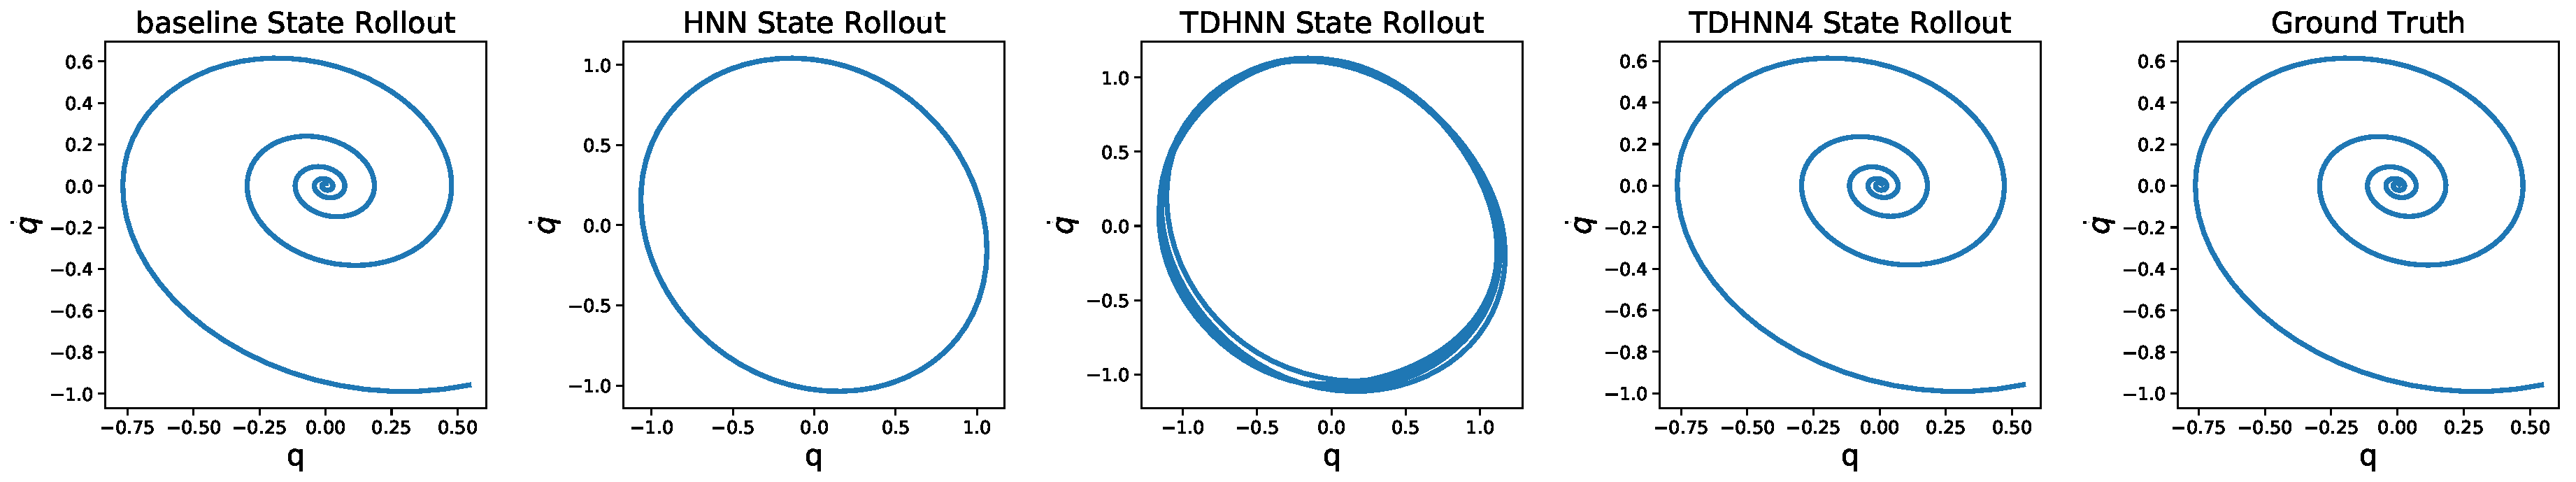
\includegraphics[width=0.4\textwidth]{figures/damped_rollout.pdf}
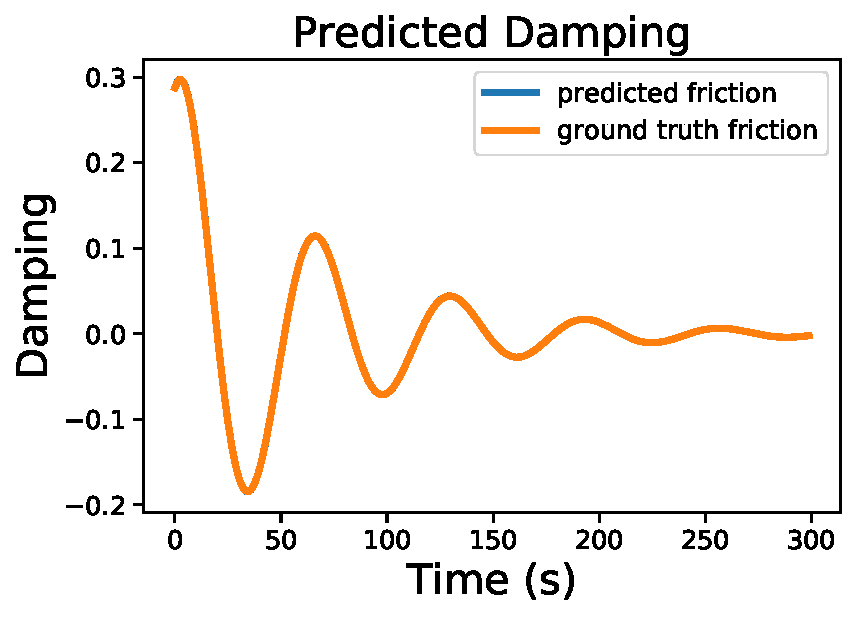
\includegraphics[width=0.4\textwidth]{figures/TDHNN4_damped_1.pdf}
\caption{Forced mass spring setting: HNN cannot learn the underlying dynamics as it has no explicit-time dependence. TDHNN4 shows the best performance as it explicitly learns a time-dependent force.}
\end{figure}

We can see that both baseline NN and TDHNN4 recover the dynamics well, whereas HNN and TDHNN struggle to learn the damping.

\subsection{Forced Mass Spring}

 We study 2 types of forced mass-spring systems. The first has the following Hamiltonian form:

\begin{equation}
\mathcal{H} = \frac{1}{2}kq^2 + \frac{1}{2m}p^2 - qF_0sin(\omega t) 
\end{equation}

\begin{figure}[h!]
\centering
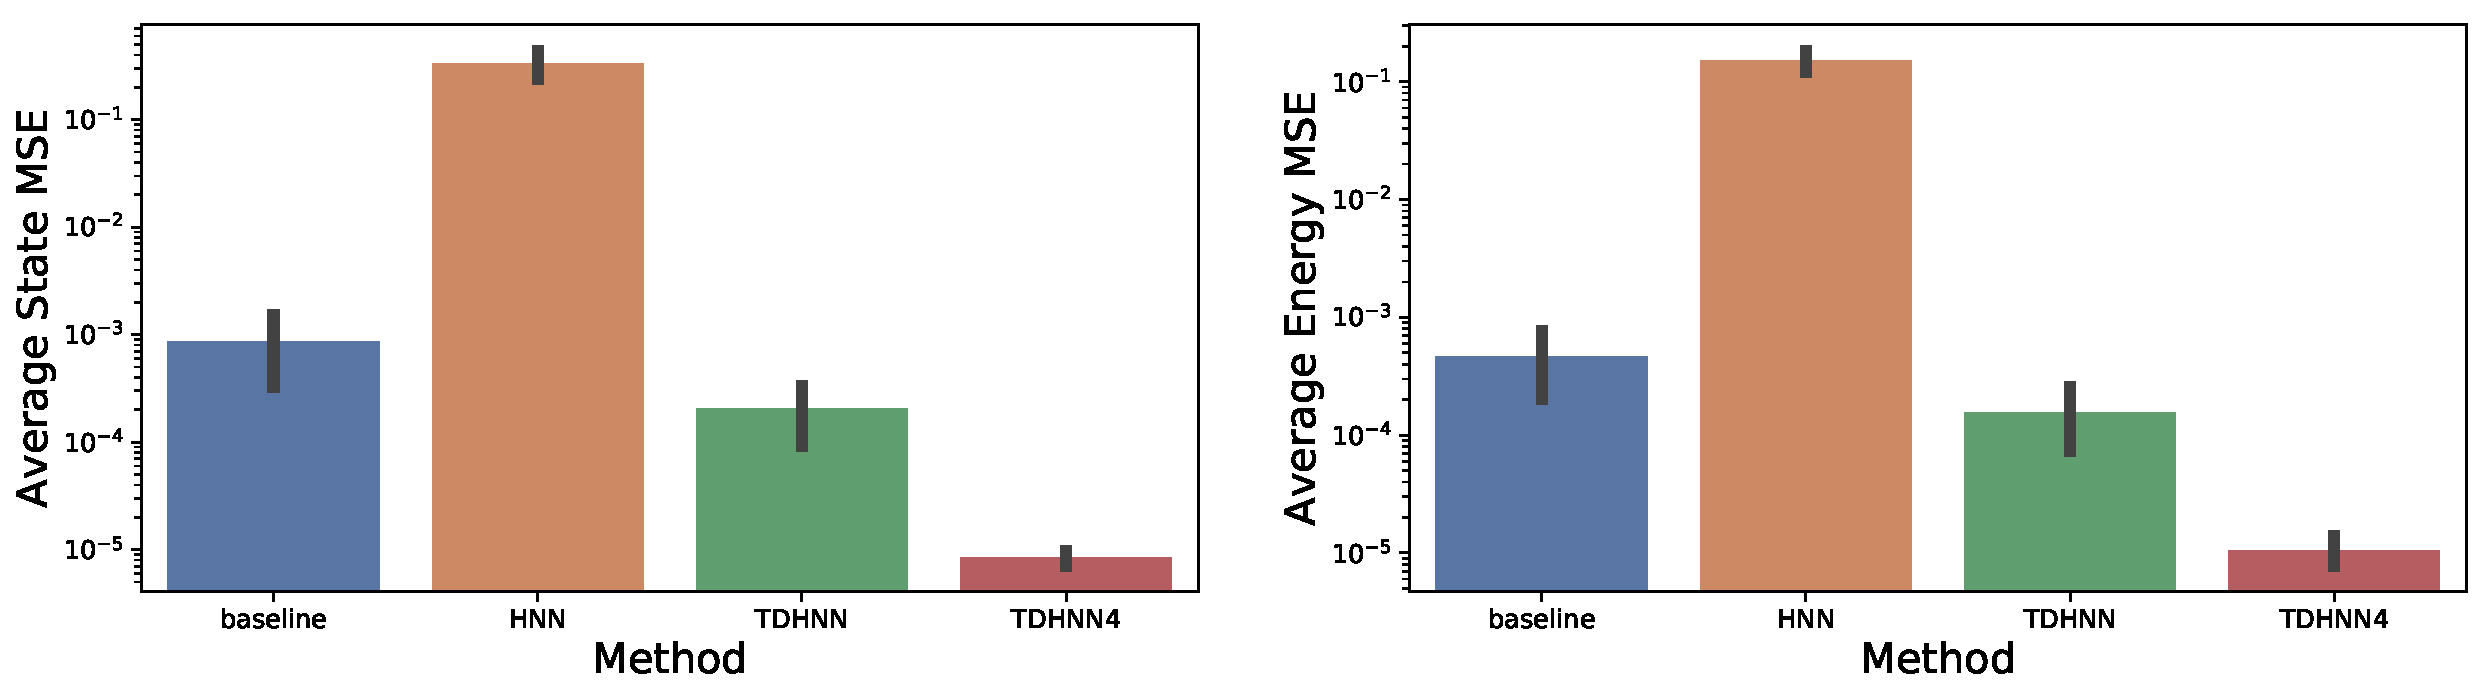
\includegraphics[width=0.5\textwidth]{figures/mass_spring_forced_1_errors.pdf}
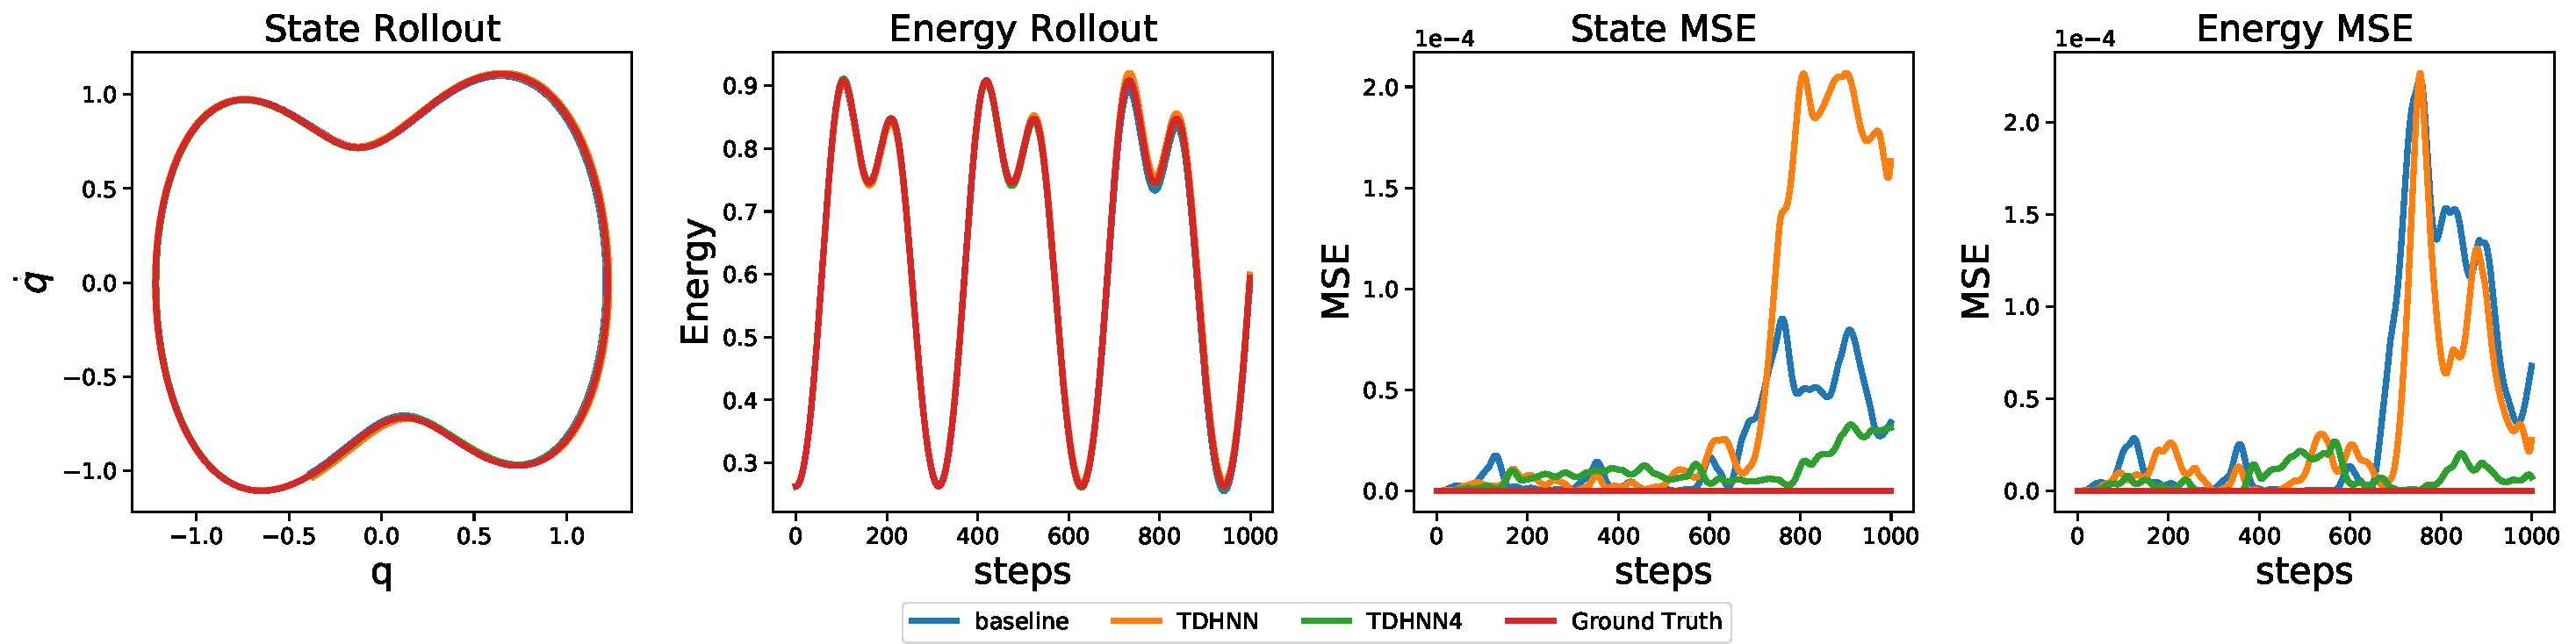
\includegraphics[width=0.4\textwidth]{figures/mass_spring_forced_1_pred.pdf}
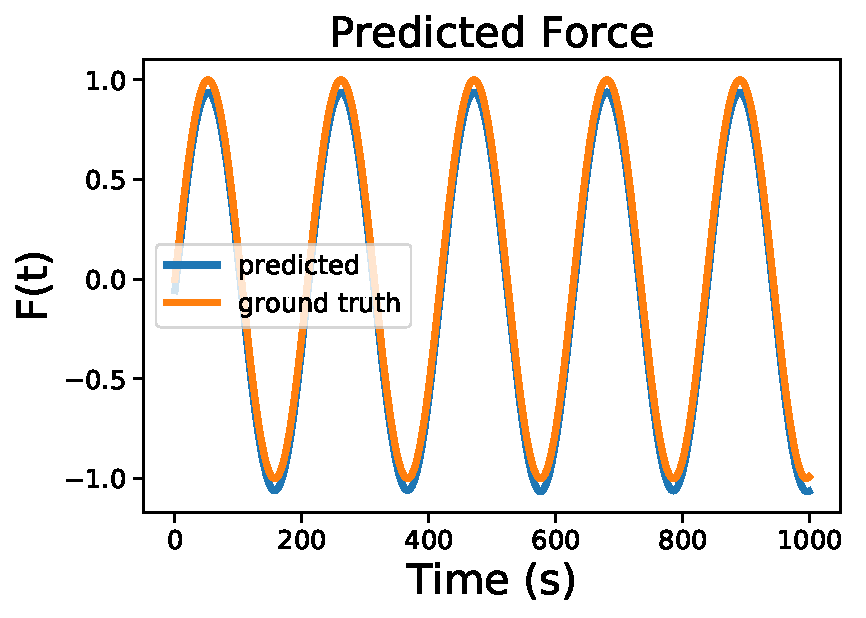
\includegraphics[width=0.4\textwidth]{figures/TDHNN4_mass_spring_force_1.pdf}
\caption{Forced mass spring setting: HNN cannot learn the underlying dynamics as it has no explicit-time dependence. TDHNN4 shows the best performance as it explicitly learns a time-dependent force.}
\end{figure}

The second has this Hamiltonian form:

\begin{equation}
\mathcal{H} = \frac{1}{2}kq^2 + \frac{1}{2m}p^2 - qF_0sin(\omega t)sin(2\omega t)
\end{equation}

\begin{figure}[h!]
\centering
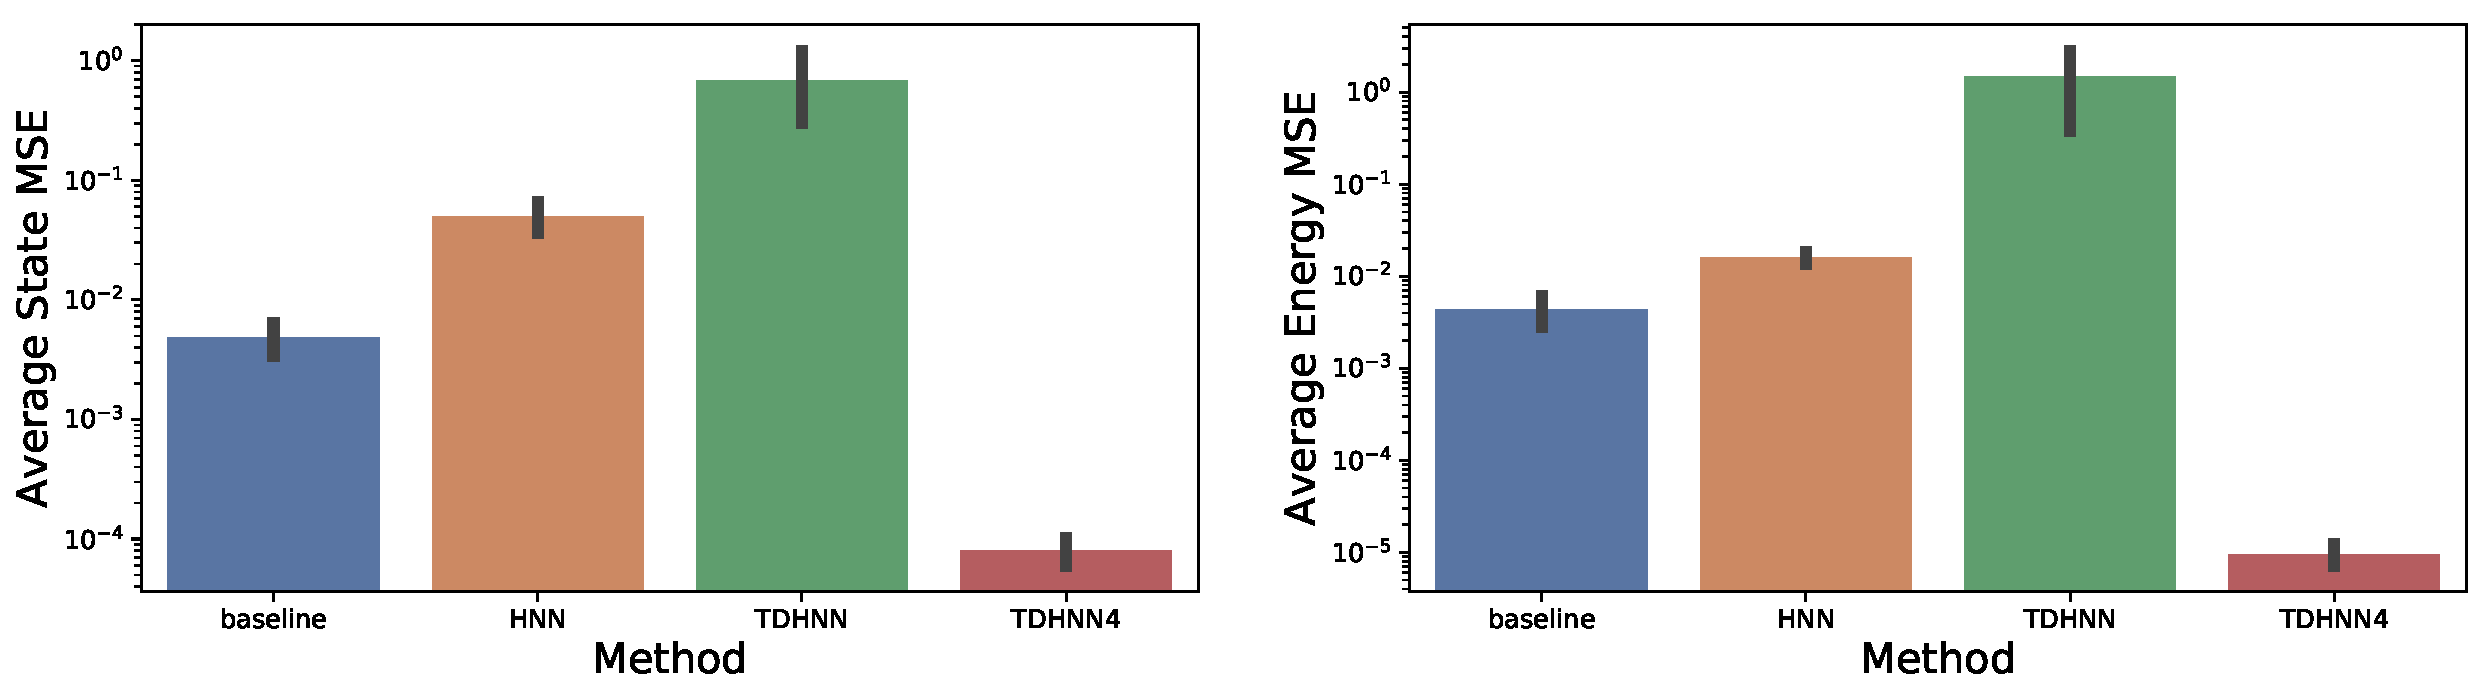
\includegraphics[width=0.5\textwidth]{figures/mass_spring_forced_2_errors.pdf}
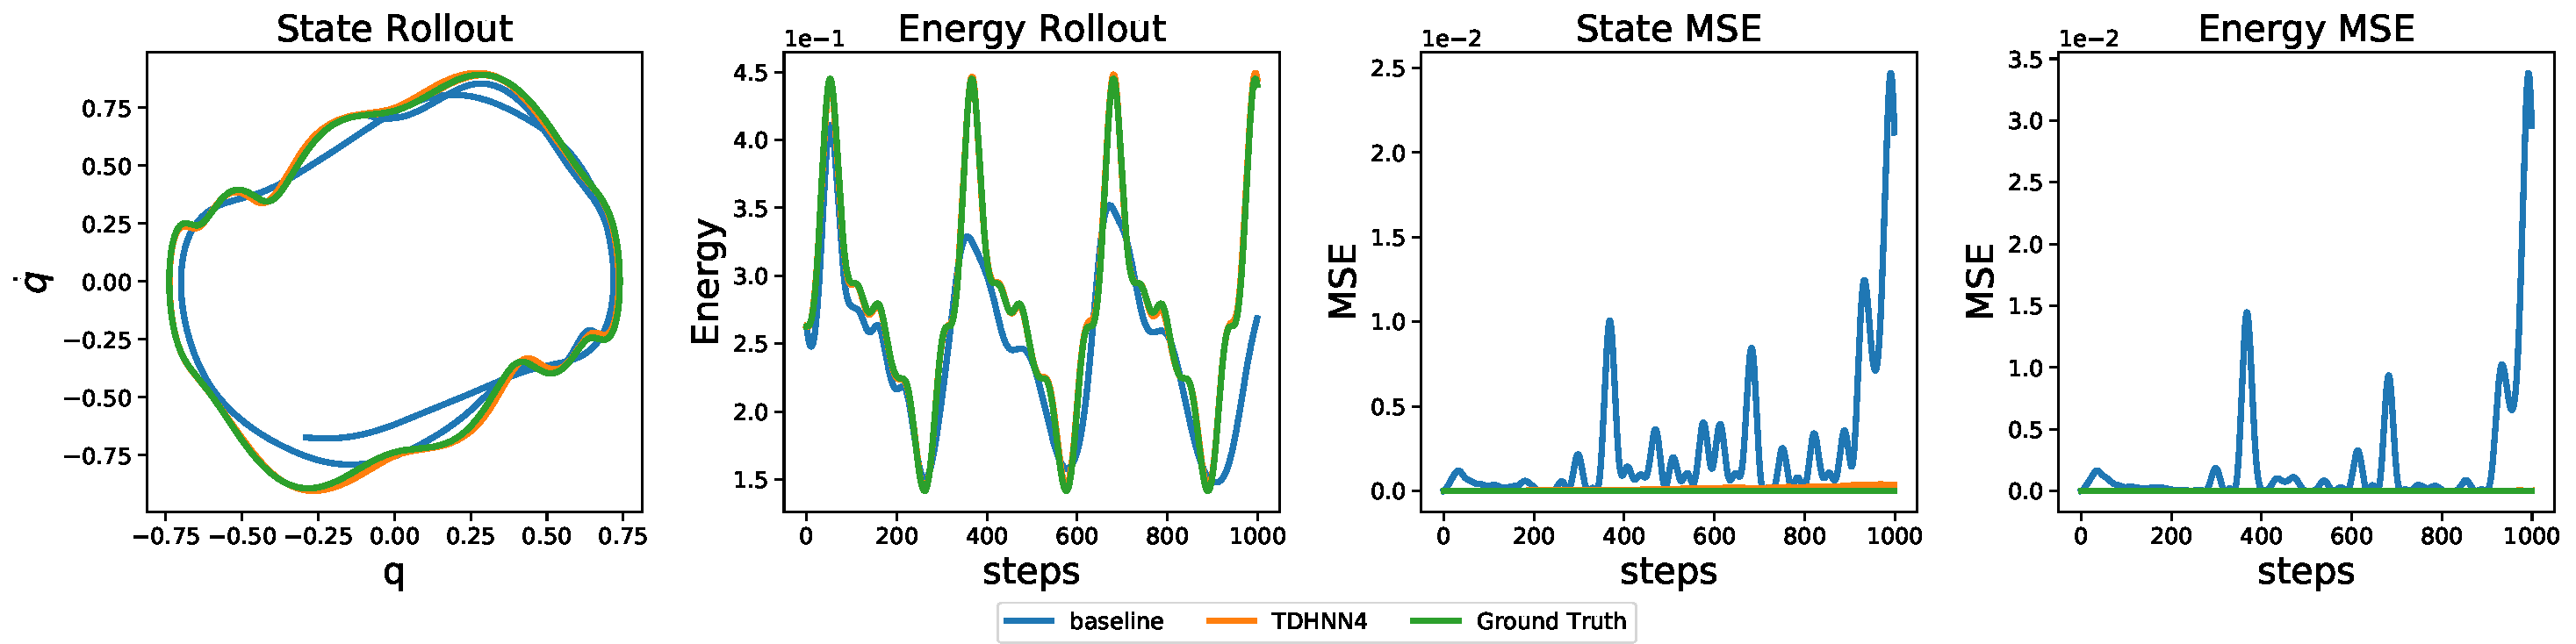
\includegraphics[width=0.4\textwidth]{figures/mass_spring_forced_2_pred.pdf}
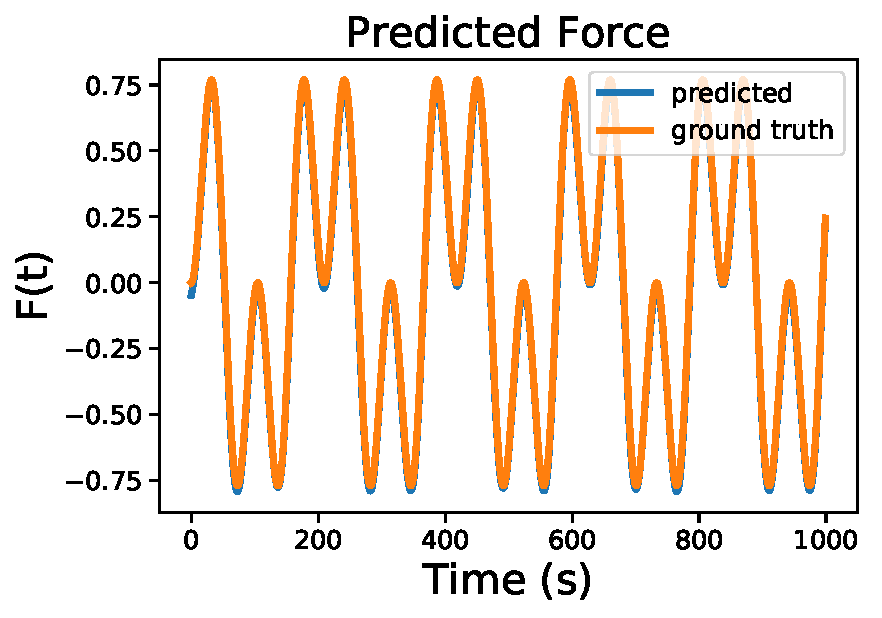
\includegraphics[width=0.4\textwidth]{figures/TDHNN4_mass_spring_force_2.pdf}
\caption{The time dependent force here is non-trivial, but TDHNN4 shows it can recover it precisely.}
\end{figure}

\subsection{Duffing}

The general duffing equation combines both the force and damping terms. Typically the equation is written as:

\begin{equation}
\ddot{\mathbf{q}} = -\delta \dot{\mathbf{q}} -\alpha \mathbf{q} -\beta \mathbf{q}^3 +\gamma \sin(\omega \mathbf{t}) 
\end{equation}

One can see that the unforced and undamped regular Hamiltonian of the duffing system would be:

\begin{equation}
\mathcal{H}_{reg} = \frac{\mathbf{p}^2}{2m}+ \alpha \frac{\mathbf{q}^2}{2} + \beta \frac{\mathbf{q}^4}{4}
\end{equation}

This Hamiltonian therefore has a potential that would either be a single or a double well.


\subsubsection{Non-Chaotic}

Given a set of initial parameters where $\alpha =-1,\beta=1,\delta=0.3,\gamma=0.2,\omega=1.2$ we can obtain training data for the non-chaotic regime of the duffing equation.

\begin{figure}[h!]
\centering
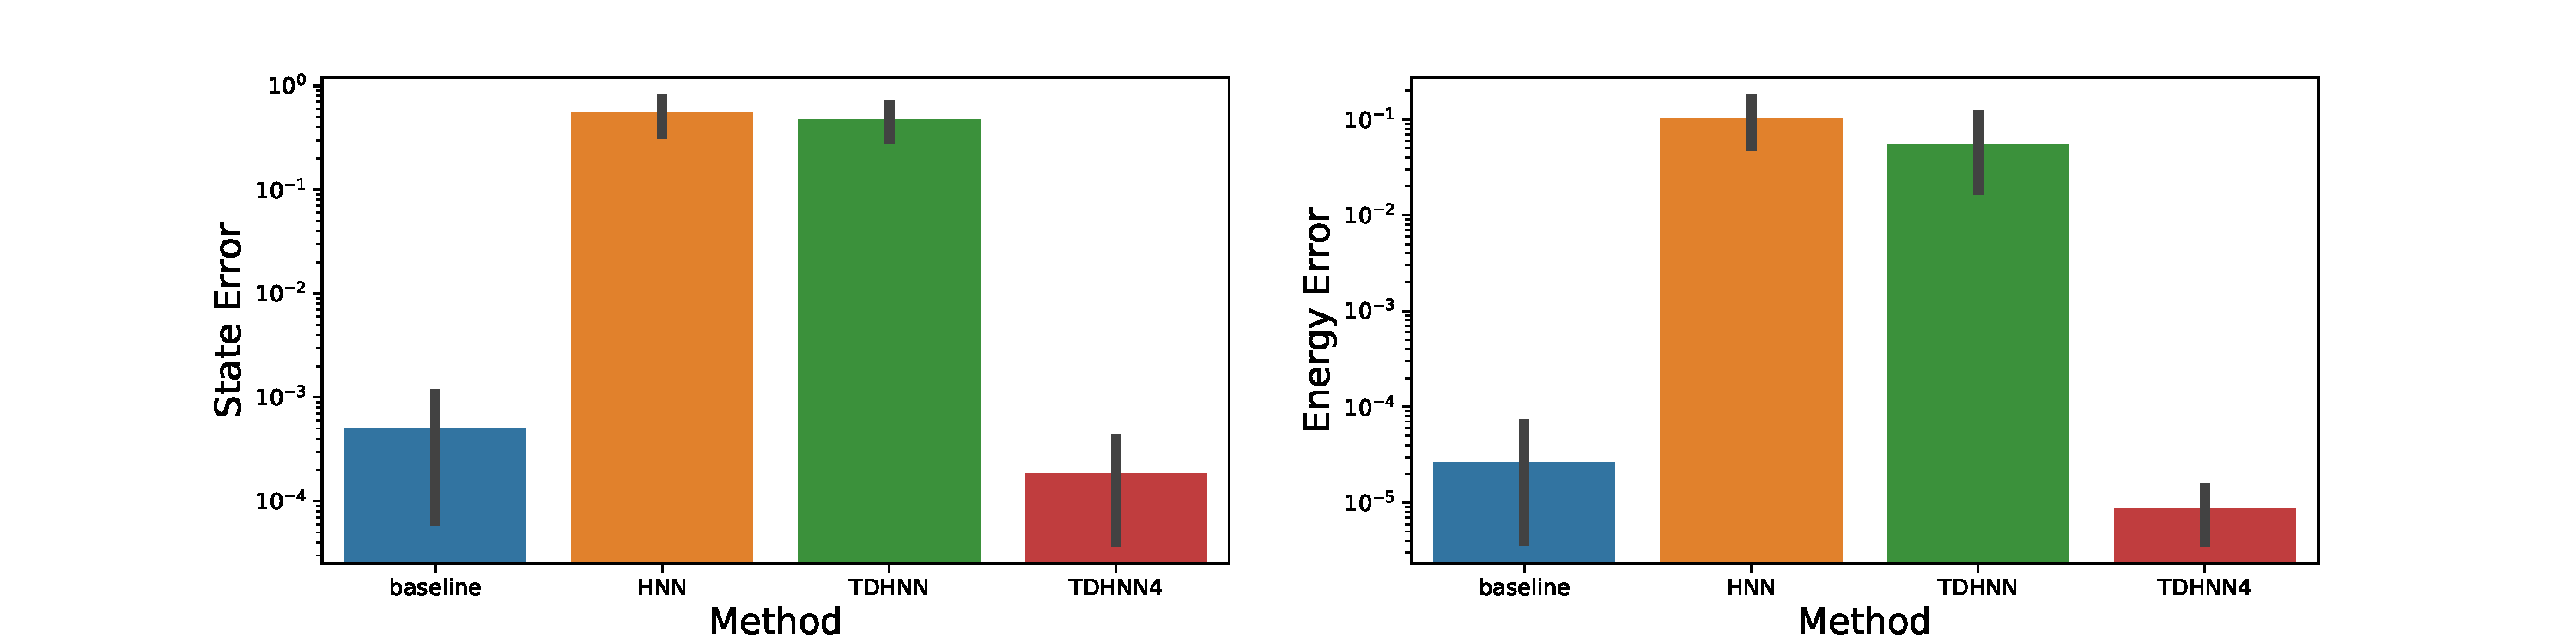
\includegraphics[width=0.5\textwidth]{figures/duffing_1_errors.pdf}
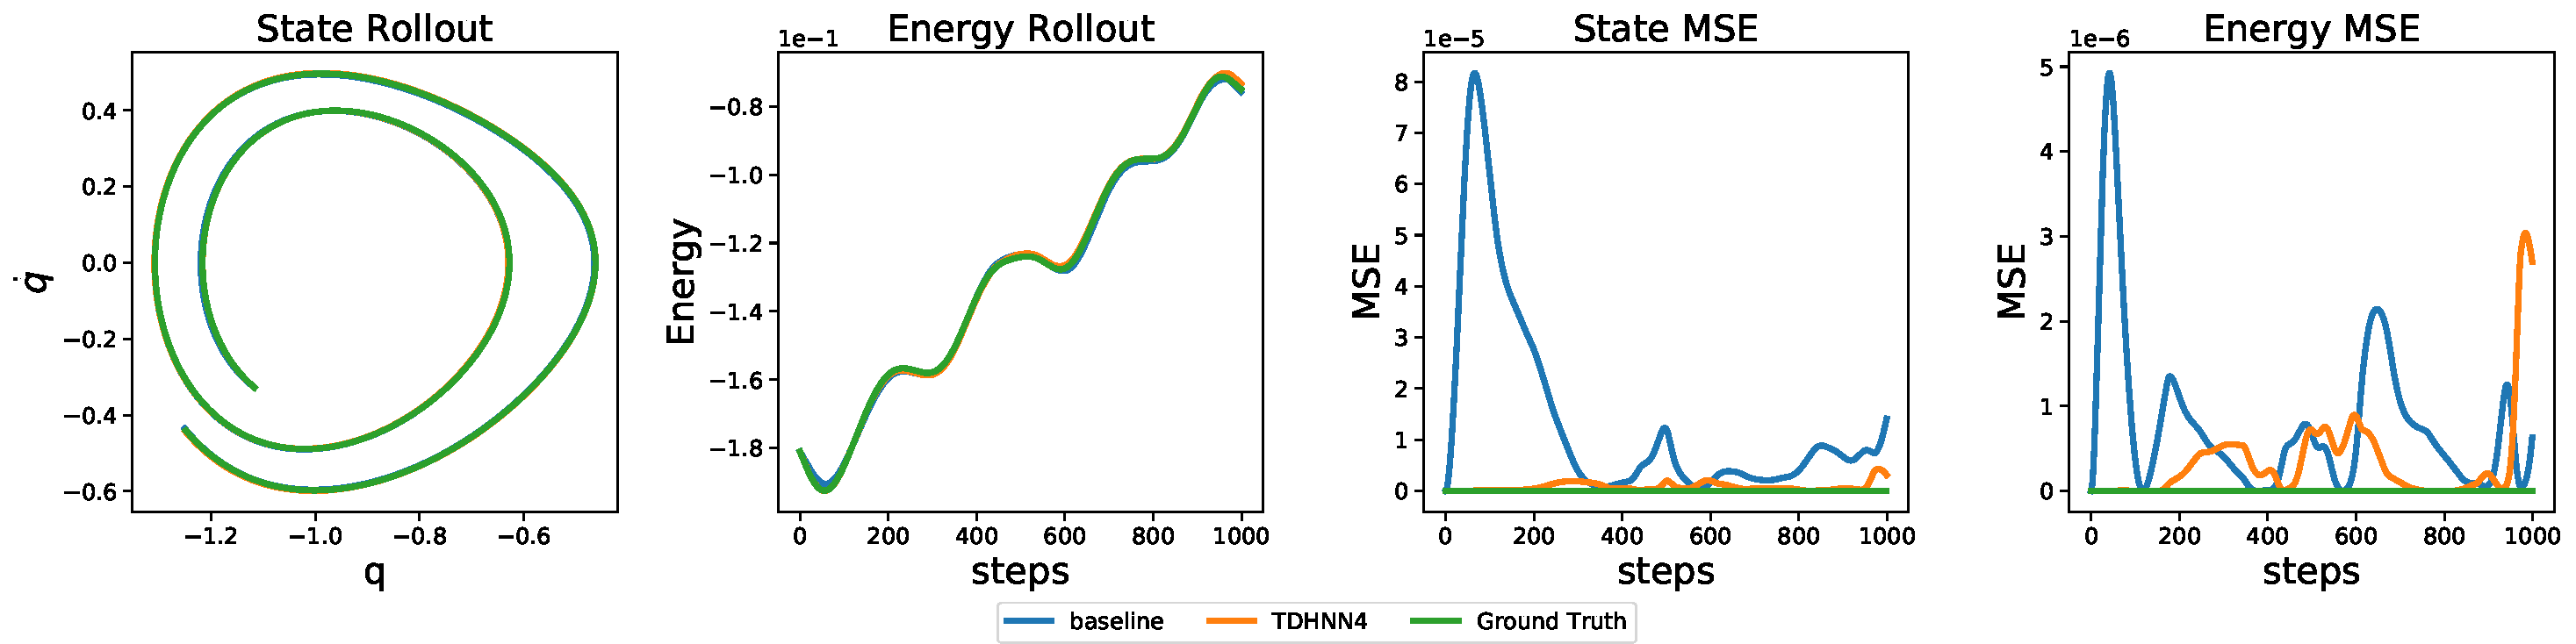
\includegraphics[width=0.4\textwidth]{figures/duffing_1_pred.pdf}
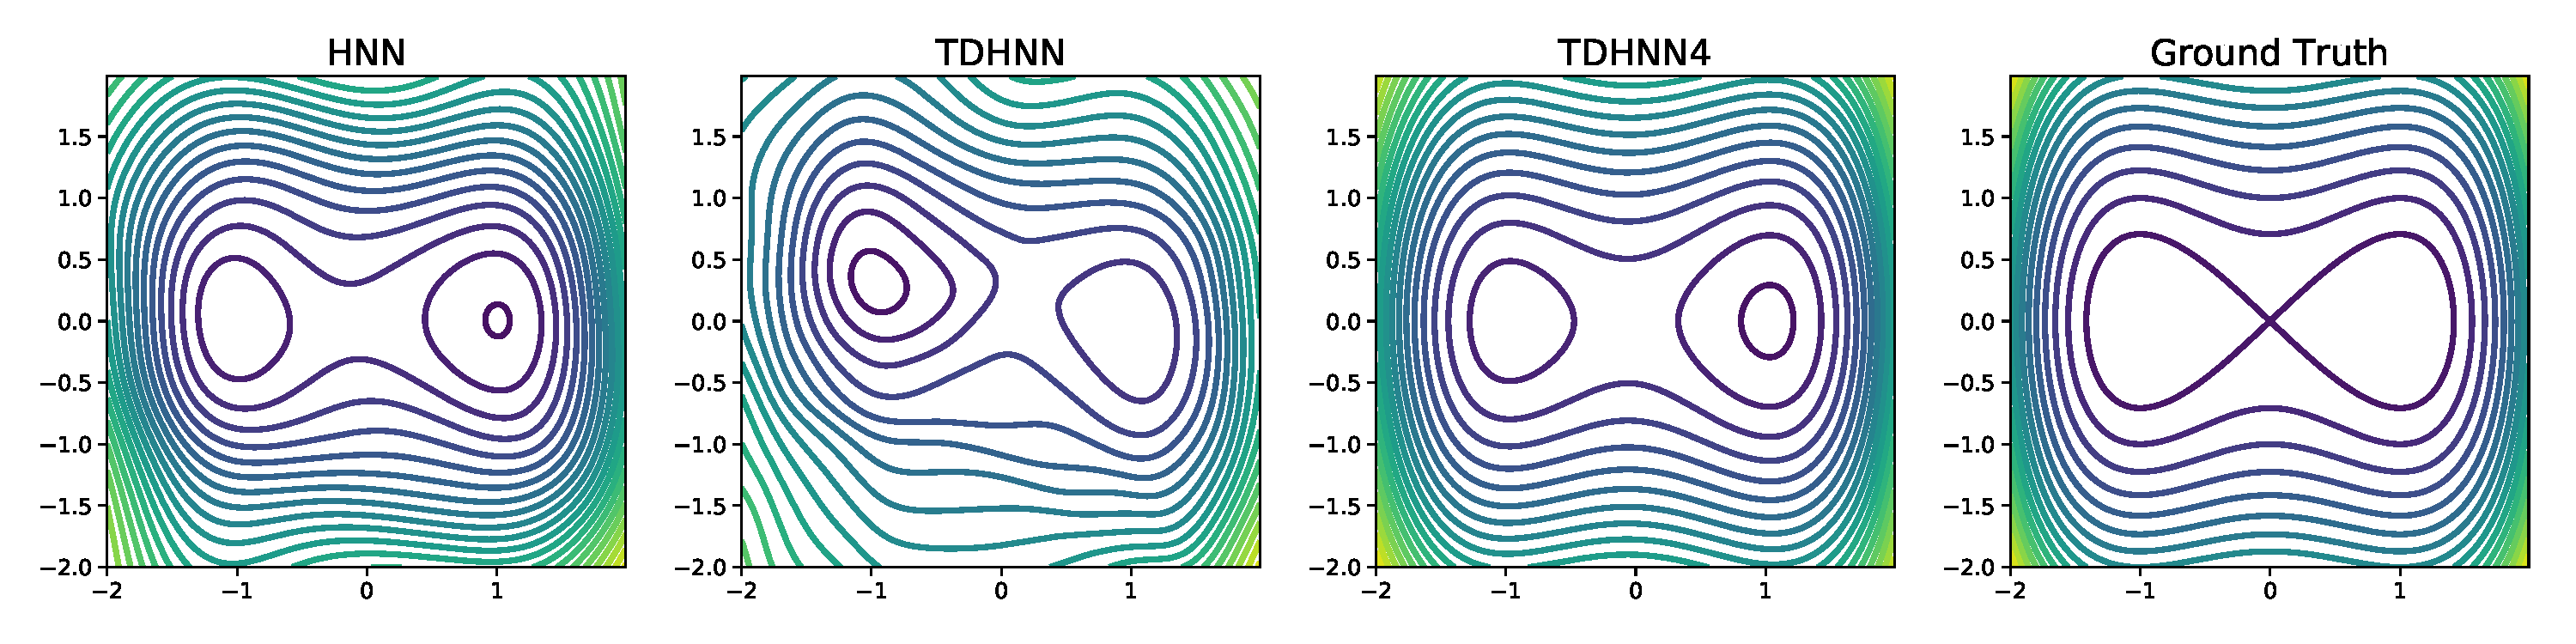
\includegraphics[width=0.4\textwidth]{figures/duffing_ham_1.pdf}
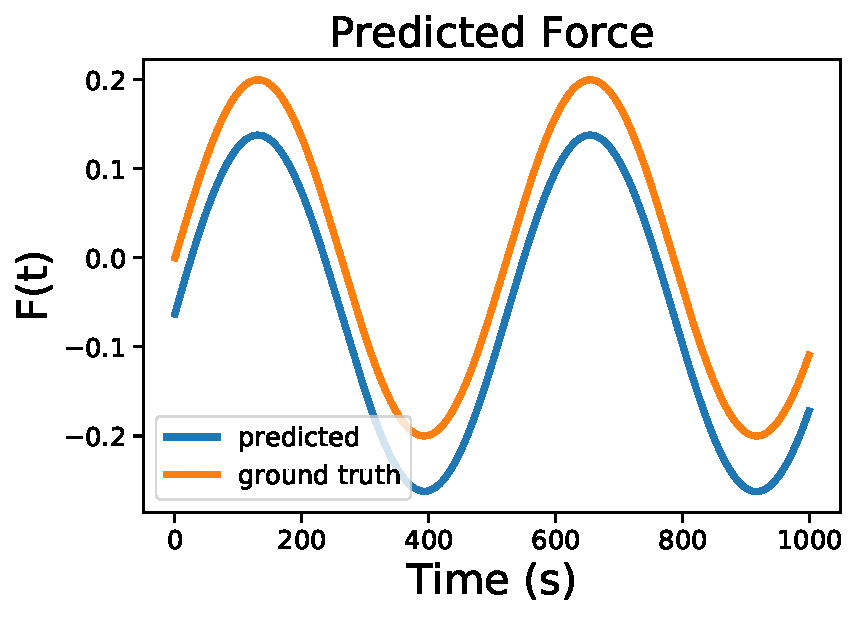
\includegraphics[width=0.4\textwidth]{figures/TDHNN4_duffing_1.pdf}
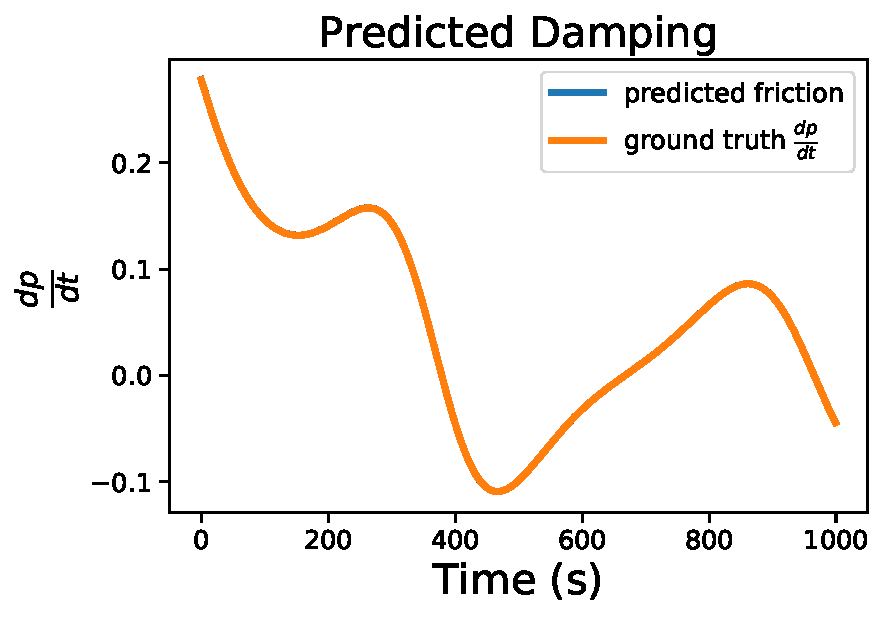
\includegraphics[width=0.4\textwidth]{figures/TDHNN4_duffing_damp_1.pdf}
\caption{baseline NN and TDHNN4 both perform really well in this setting. With TDHNN4 we are also able to extract the ground truth force and damping coefficient. The predicted Hamiltonian also visually appears closer to the ground truth in comparison to HNN or TDHNN.}
\end{figure}

\subsubsection{Chaotic}

In the chaotic regime we use the following parameters:
$\alpha =1,\beta=1,\delta=0.1,\gamma=0.39,\omega=1.4$. 

Training Data: 20 initial conditions, sampled uniformly in $[-1,1]^2$ each rolled out for one period $T=2\pi/\omega$ where $\delta t = T/100$. This results in 2000 training points.

Testing: we test the system on a single initial condition, rolled out to $T_{max} = 18,000$ with the same $\delta t$ as training. One additional change we make at inference is a modification to the time variable which is fed in. We work under the assumption that we have explicit knowledge of the period, and as such, we modulo the time variable with the period. This is necessary as the models are not explicitly trained on time steps beyond $T$. Using the unchanged time, our model predictions rapidly diverge from the ground truth. Our results are visually presented in Fig.\ref{fig.chaos}.  
\subsection{Relativity}



\begin{table*}[ht!]
\caption{Test Rollout MSE} 
\centering % centering table
\resizebox{\textwidth}{!}{\begin{tabular}{c  cc cc cc cc cc} % creating eight columns
\hline\hline %inserting double-line
\multirow{2}{*}{Method}&\multicolumn{2}{c}{Ideal Mass Spring}&\multicolumn{2}{c}{Damped Mass Spring} & \multicolumn{2}{c}{Forced Mass Spring (1)} &\multicolumn{2}{c}{Forced Mass Spring (2)} & \multicolumn{2}{c}{Duffing Non-Chaotic} \\
\cline{2-11} % inserts single-line
 & State & Energy & State & Energy & State & Energy & State & Energy & State & Energy \\
\hline
Baseline NN &\\ % Entering row contents
HNN &\\
TDHNN &\\
TDHNN4 &
\\% [1ex] adds vertical space
\hline % inserts single-line
\end{tabular}}
\label{tab:tests}
\end{table*}

\pagebreak

\bibliography{references.bib}
\end{document}
